\documentclass{article}

\usepackage{url}
\usepackage{graphicx}
\usepackage{babel,blindtext}
\usepackage{float}
\usepackage{hyperref}
\hypersetup{
    colorlinks=true,
    linkcolor=black,
    filecolor=black,
    urlcolor=black,
    citecolor=black,
}

% Default margins are too wide all the way around. I reset them here
\setlength{\topmargin}{-.5in}
\setlength{\textheight}{9in}
\setlength{\oddsidemargin}{.125in}
\setlength{\textwidth}{6.25in}

\begin{document}

\title{Ear Recognizer Android}
\author{Leonardo Emili, Alessio Luciani\\
Sapienza University of Rome}
\renewcommand{\today}{February, 2021}
\maketitle

\section{Introduction}

The ear as a new biometrics has recently gained a discrete success because of some fundamental properties it has,
among them: uniqueness, permanence, collectability, and universality.
We owe A. Iannarelli for these incredibile findings, in 1989 he discovered that no pair of individuals
share the same ear shape, therefore it is possible to use them to identify people. Although humans are
not used to recognizing people by their ear shape, it is possible to leverage a number of keypoints
(namely points of interest) in the ear shape in order to distinguish them. Moreover, ears present
less details with respect to other biometrics (e.g. the face), hence allowing them be captured by
means of lower resolution devices. However, some challenges must be tackled when dealing with ear
recognition: the size and the fact that they share the same colour of the skin puts some difficulties,
as well as their position that may be an obstacle because they may be only partially visible.
In the years, researchers proposed several approaches to deal with the ear recognition task, in some
cases requiring the use of complex neural networks as well as a large collection of annotated data
to train them. In this work, we implemented a recognition system according to the best pratices that
are adopted when designing a biometric module, exploring different techniques that are currently employed
by state-of-the-art solutions.

\section{Dataset}

We conducted our experiments using the Mathematical Analysis of Images (AMI) Ear Database \cite{ami}: it consists
of a collection of 700 2D images acquired from 100 different subjects in an indoor environment.
Images show a high degree of variability since they represent ears of subjects in the range of 19-65 ears
taken from multiple points of view. Since all of the images come shipped with the identifier of the subject
they belong to, we have been able to evaluate our work against it and draw some considerations
about the final performances.

\section{Localization phase}

The first step of the pipeline aims at designing a detection module for detecting whether the provided image
contains ear shapes or not and for localizing their position within the image. The idea is that we only care
about portions of the original image containing ears while discarding other irrelevant information.
From now on, we will refer to these portions with the term of Region of Interest (ROI), denoting the bounding
box surrounding the ear zone. Our goal is to build a detection module that is robust enough to rotations,
translations, viewpoint, and scale changes. The reason is that images may not be perfect and the ear region
not perfectly centered, but we want to be able to extract valid ROI no matter their position in the original
image. To this aim, we relied on Viola-Jones Haar Feature-based Cascade Classifiers \cite{conf/cvpr/ViolaJ01}
to detect valid ROI.
The algorithm works by combining the power of Haar-like features to useful extract information from the
image (e.g. presence of edges or straight lines) with the concept of integral images to speed up computations.
The AdaBoost algorithm is responsible for the training procedure which selects a subset of meaningful features
from the original set of features. Finally, a sequence of gradually stronger classifiers is applied over the
input image to detect if it contains an ear shape. If at any stage, the decision is negative then the considered
window is discarded without any further processing.

\begin{figure}[h]
    \label{fig:detection}
    \begin{center}
        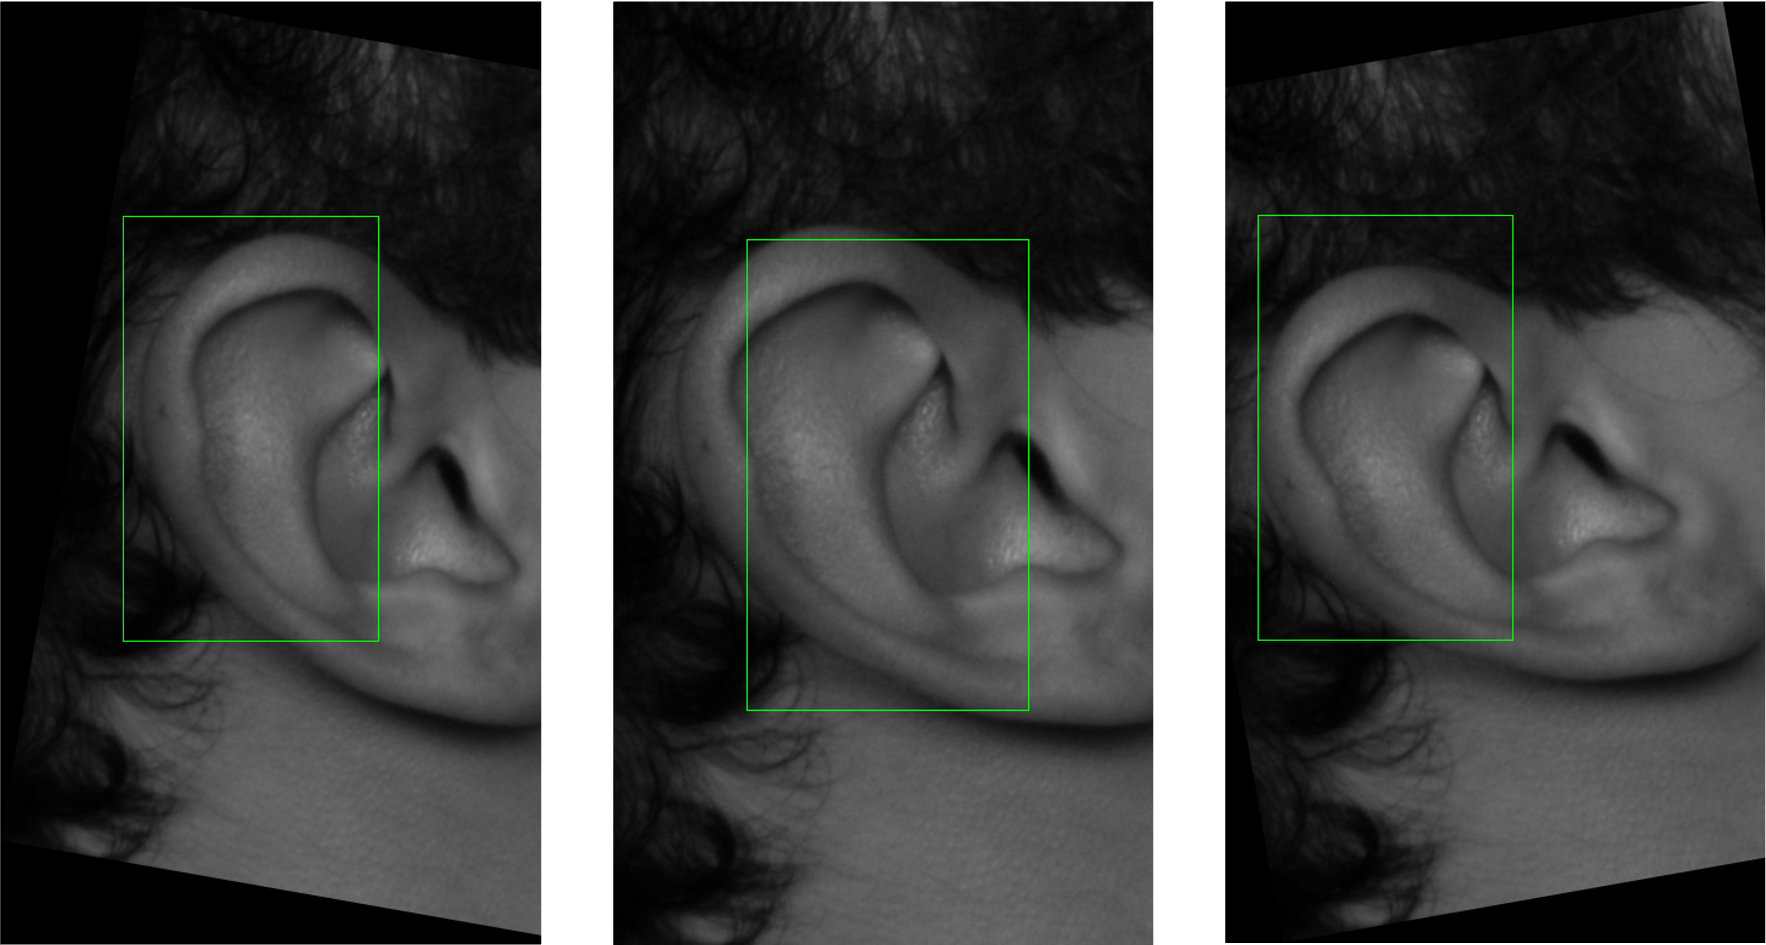
\includegraphics[width=10cm,keepaspectratio]{images/detection.png}
        \caption{ROI after applying a degree of rotation (-10/0/+10°).}
    \end{center}
\end{figure}

In the above figure, it is possible to see the effects of applying ear detection on a real image from the
dataset. It is clear that the best localization results are achieved when the image is not rotated at all.
However, it is worth noting that the bounding box denoted by the detection procedure does not contain the
whole ear and cuts off some external regions.  For the sake of completeness, we also include the results when
a small rotation is applied to the image. We can see that the ear zone localization is still quite good even
though the aforementioned problem is more evident.
In order to improve the quality of the localization performed by the considered classifiers \cite{Castrillon11-caepia},
we propose a slight modification of the original algorithm
where the considered ROI is the bounding box returned by the algorithm plus a small area of padding of size
$k$ around it. We experimentally found that for $k=80$ our model performs the best and below here we can
see that previous issues are less visible:

\begin{figure}[h]
    \label{fig:padding_detection}
    \begin{center}
        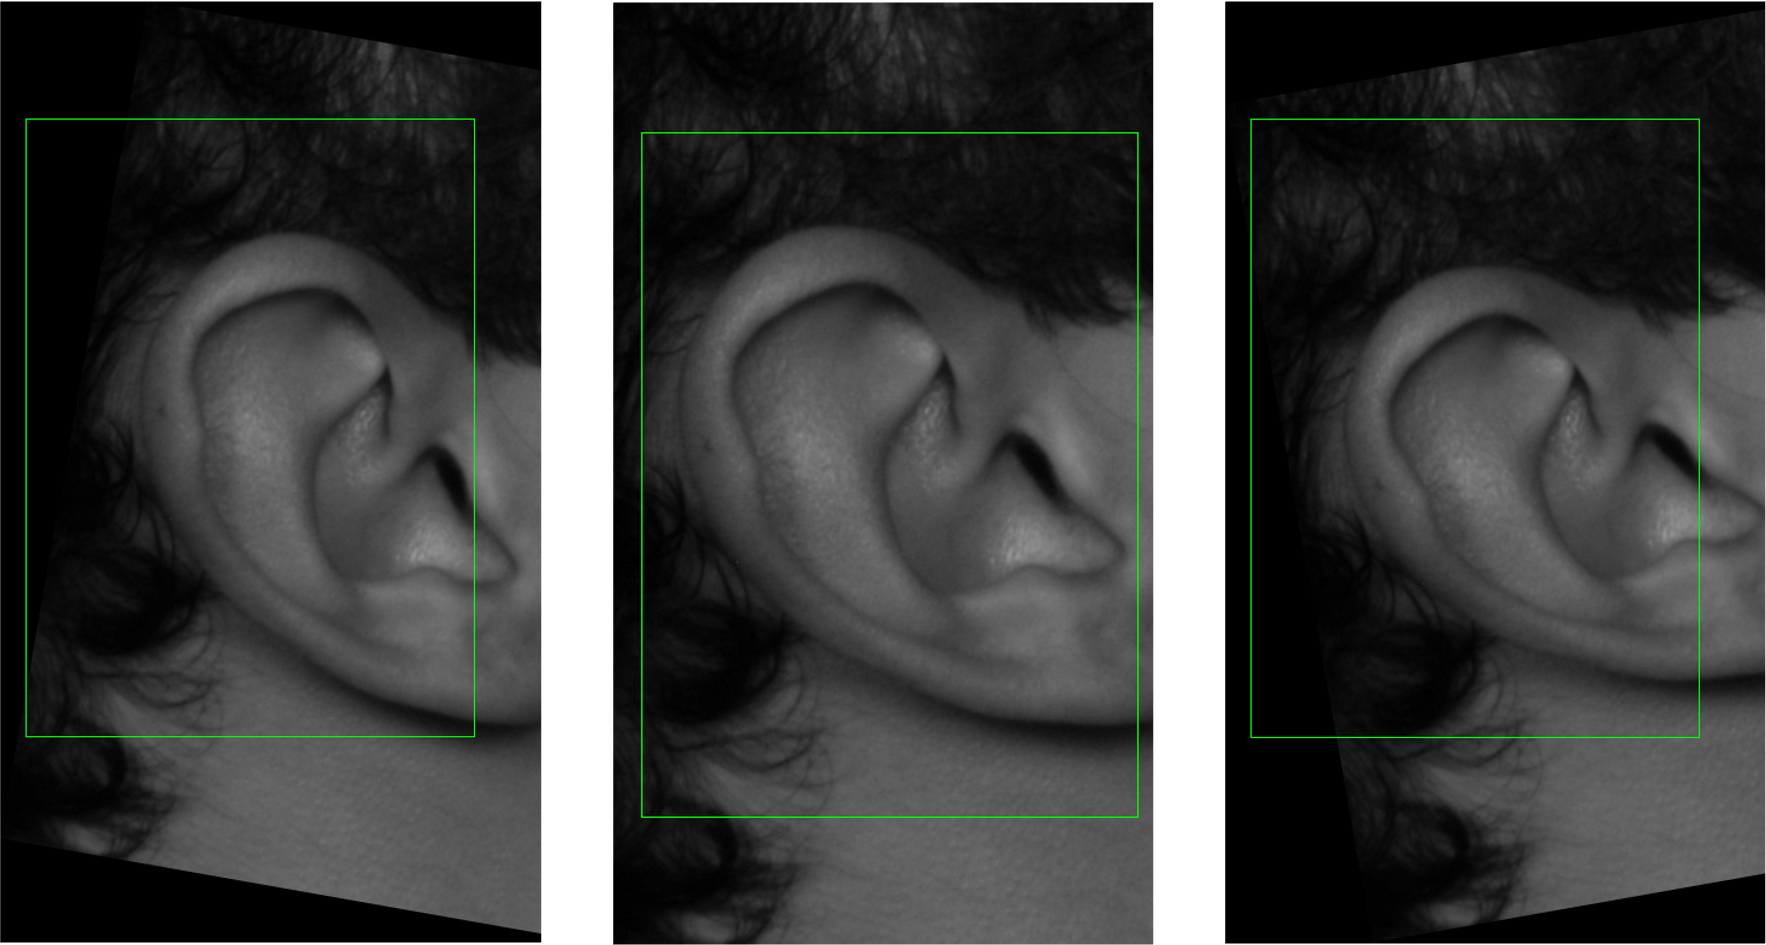
\includegraphics[width=10cm,keepaspectratio]{images/padding_detection.png}
        \caption{ROI with padding after applying a degree of rotation (-10/0/+10°).}
    \end{center}
\end{figure}

Since the AMI dataset contains images of left ears as well as right ears, we decided to only keep images
of left ears to facilitate the later matching step. In particular, we manage to get the ROI by applying
both the left and right cascade classifier on the original image and finally flip it over the vertical
axis if the image represents a right ear. By doing so, we obtain a detection rate of 54.45\% and proceed
with the rest of the pipeline on the detected images.
At the end of this phase, we finally have our ROI, and by cropping the green areas,
we can ignore the rest of the image. It is worth noting that all the images are converted into
grayscale images and resized into a fixed size for the next steps.

\section{Landmark detection phase}

In this phase, we explored some of the most common approaches when extracting points
of interest (i.e. landmarks). We first experimented using a state-of-the-art convolutional neural network
(CNN) from the work of Hansley et al. that was specifically trained on this task and it performed quite well.

\begin{figure}[h]
    \label{fig:landmark}
    \begin{center}
        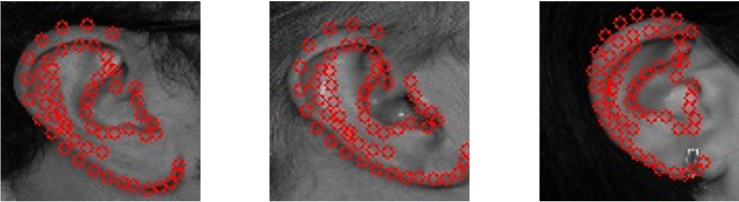
\includegraphics[width=12cm,keepaspectratio]{images/landmark2.png}
        \caption{Landmark detection using a state-of-the-art CNN.}
    \end{center}
\end{figure}

However, for the aim of this project, we thought that it would be interesting to test ourselves
by experimenting with some specific algorithm instead of using an off-the-shelf model. In this context,
we analyze the effects of applying the Oriented FAST and rotated BRIEF (ORB) algorithm \cite{conf/iccv/RubleeRKB11}
for detecting
image keypoints and extracting features. The algorithm essentially works by combining the feature detection
provided by the FAST algorithm \cite{rosten_2006_machine}, which performs corner detection by inspecting if a pixel
has a contiguous
set of pixels that are brighter or darker than a threshold, and the BRIEF algorithm \cite{Calonder:2010:BBR:1888089.1888148}
for feature description
computation, which allows us to get a compact feature vector. It's important to say that the two
algorithms are used in this context for the same purpose (i.e. landmark detection), but their task is
slightly different: while the CNN was specifically trained for detecting landmarks that are specific to ear
shapes, the ORB algorithm plays in a different way and aims at finding generic image keypoints. Thus,
we expect the resulting set of keypoints to be different from each other.

\begin{figure}[h]
    \label{fig:landmark_orb}
    \begin{center}
        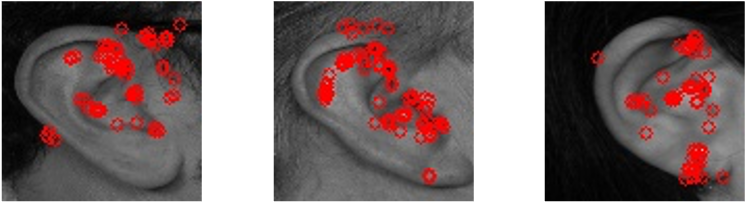
\includegraphics[width=12cm,keepaspectratio]{images/landmark_orb.png}
        \caption{Landmark detection using the ORB algorithm.}
    \end{center}
\end{figure}

We can see how the set of landmarks produced by the ORB algorithm is much more widespread around the
center of the ear and does not necessarily follow the ear shape. However, we thought we could improve the
results achieved using ORB by doing some considerations about the distribution of our data. We know that the ear
region contains many meaningful key points that will later be used when matching incoming probes with templates
belonging to enrolled subjects. If we inspect how these points are distributed we can clearly distinguish some
outliers (e.g. in the hair region) from the rest of the points that are concentrated around the center of the ear.
Hence, we decided to apply data reduction to our set of landmarks $X$ and only to retain those points that
satisfy the following condition:

$$ d(x_i, \mu_X) <= l * \sigma_X $$

where $d(x_i,x_j)$ is the Euclidean distance bewteen $x_i$ and $x_j$, $\mu_X$ and $\sigma_X$ are respectively the
centroid and the standard deviation of our set of points, and $l$ can be seen as a factor that controls how strictly
we are filtering out points that are far from the centroid. Here, we see the effects for different values of $l$,
where the green circles represent points that satisfy the condition while red points discarded:

\begin{figure}[h]
    \label{fig:landmark_orb_reduced}
    \begin{center}
        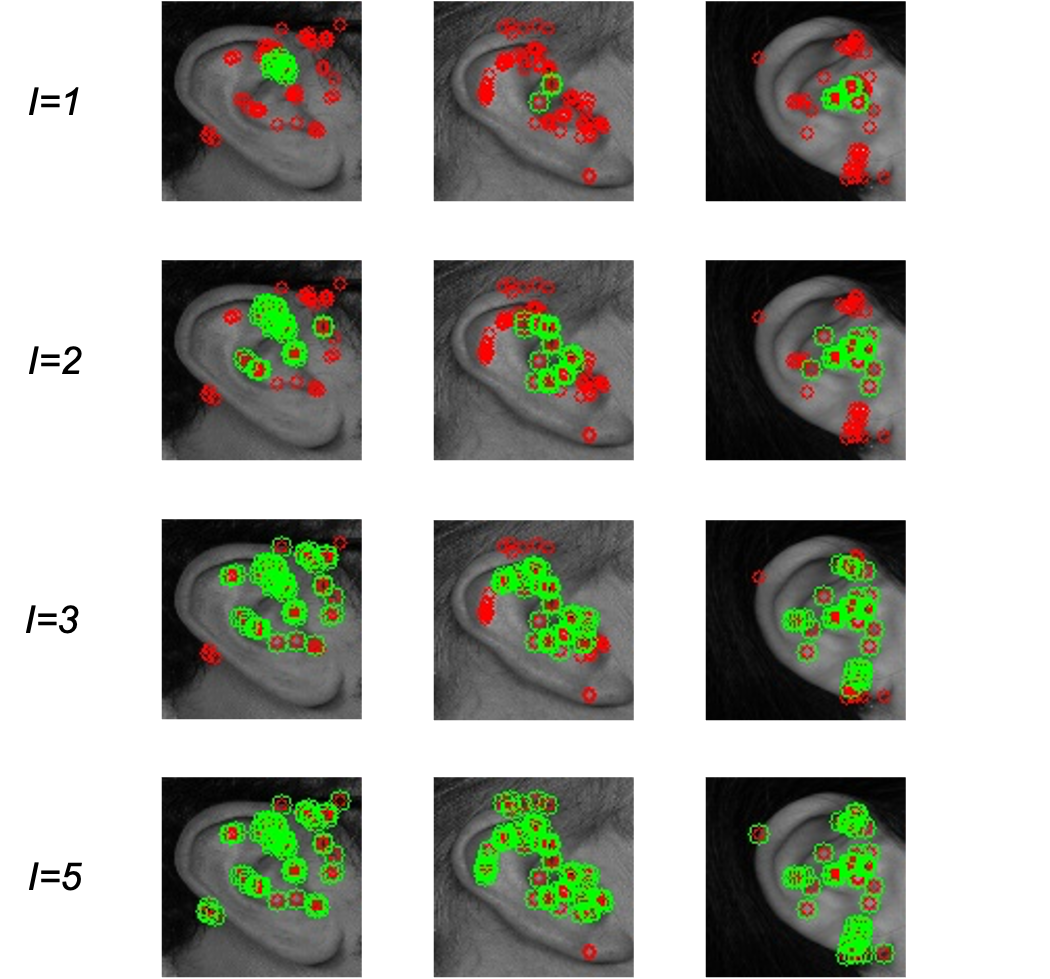
\includegraphics[width=14cm,keepaspectratio]{images/landmark_orb_reduced.png}
        \caption{Effects of landmarks reduction based on sparsity of data points.}
    \end{center}
\end{figure}

We can observe that when $l$ is low many important landmarks are discarded, on the other hand,
if we choose a suitable value for $l$ we can have a better approximation of the landmarks that were previously
obtained using a dedicated CNN. We find it particularly interesting because the latter results can be computed
much faster, and above all, we can skip the complex training and data preparation which is instead required if
using the first model.

\section{Alignment phase}

Another technique that is common when designing a biometric module is image alignment. In fact,
in the beginning, we said that we want a recognition system capable of identifying the user even if the
input probe is not perfectly centered and aligned. In order to do that, we explored a few techniques to
estimate the initial orientation of the image and we finally opted for regression. The idea is simple, if
we look at the ear shape, we can observe that it is stretched along one direction, and more interesting,
key points naturally tend to follow this direction. In these terms, we got a formulation for a linear
regression problem where the goal is to find the line that better approximates a given set of points
(i.e. the landmarks). We did it and got some unexpected results:

\begin{figure}[h]
    \label{fig:rotation}
    \begin{center}
        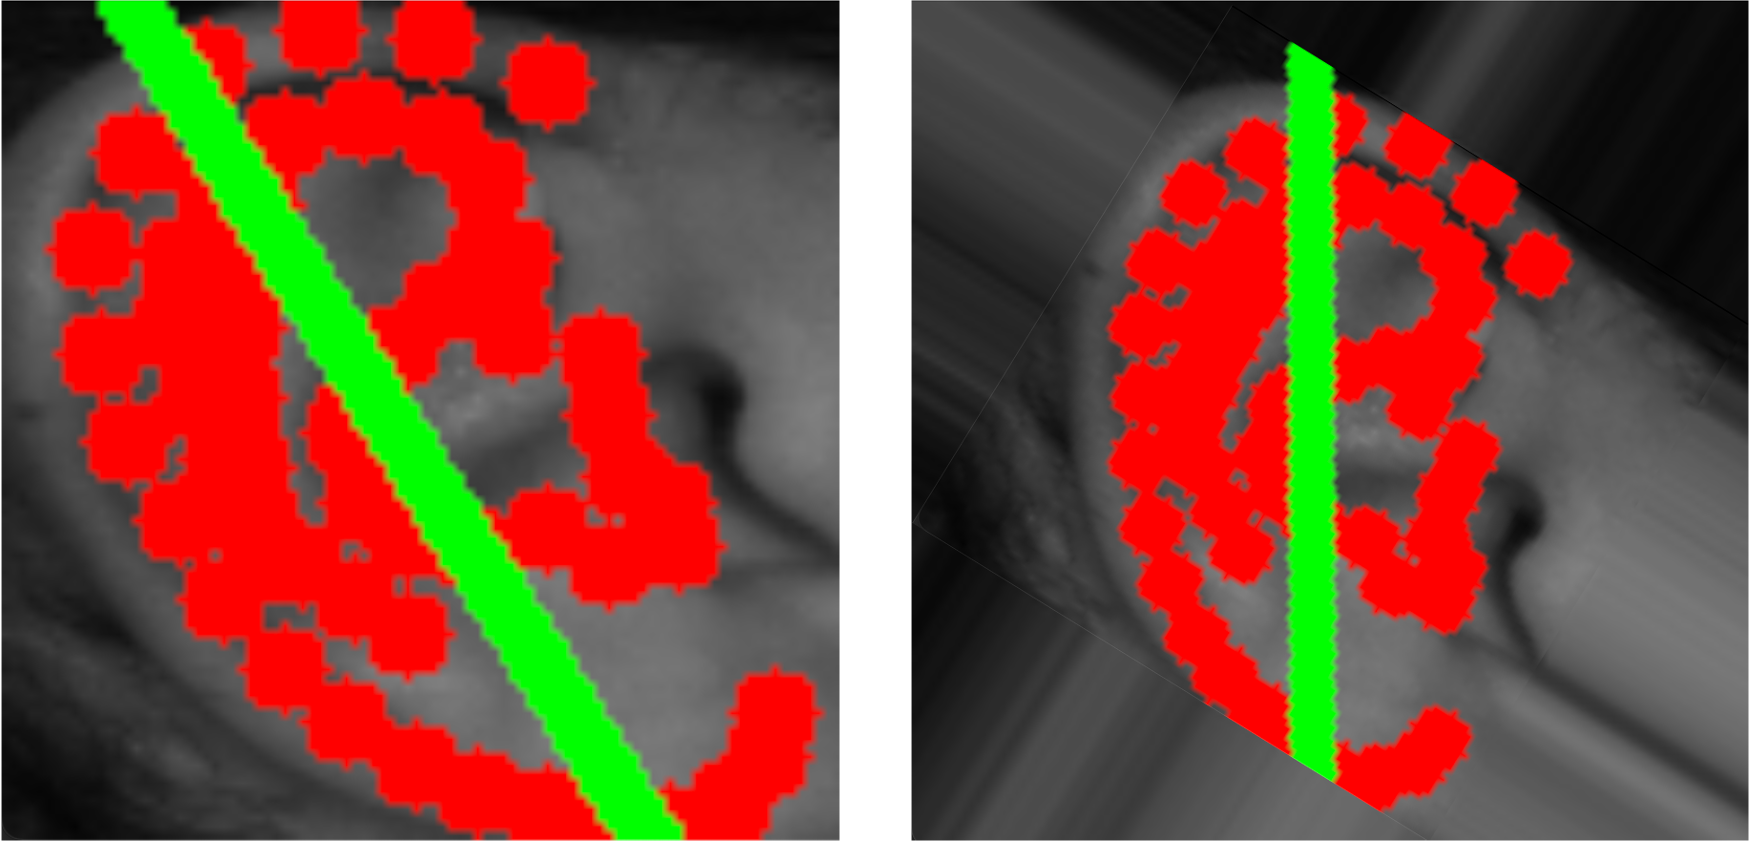
\includegraphics[width=7cm,keepaspectratio]{images/rotation.png}\\
        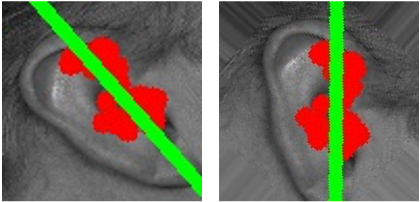
\includegraphics[width=7cm,keepaspectratio]{images/rotation2.png}
        \caption{Ear rotation using landmarks provided by the CNN vs our landmarks.}
    \end{center}
\end{figure}

As we can see, the idea of using linear regression for estimating the initial image orientation
provides us a reliable way of computing the angle $\theta$ between that line and the vertical line
that we use as a reference for our orientation system. By doing so, we are able to align all of the
images according to the compute angle, allowing a fair comparison when later we need to match the input
probe with gallery templates. 
Again, we want to precise that the set of detected landmarks produced by the two algorithms
is not the same, hence the alignment step, which is based on it, can be different choosing a
different algorithm. However, we found it interesting to see that our idea of applying linear
regression on the set of key points can be applied in both cases.
It's worth noting that rotating an image by a given angle gives us a larger
output image than the original one. In fact, with the rotation we discovered two main issues: the size
of the output image depends on the value of $\theta$ and the areas of the output image corresponding to
the corners need to be filled with some value in order to be matched with other images. The first issue
tells us that when later we will match an input probe with gallery templates, their size once processed
may be different. On the other hand, the latter happens because we consider the corners of the original
image to be part of the rotated one, but if we look closer at Figure \ref{fig:padding_detection} we can see
that they designate a
portion of the detected ROI that does not necessarily contain useful information for our matching purposes.

\begin{figure}[H]
    \label{fig:rotation_issue}
    \begin{center}
        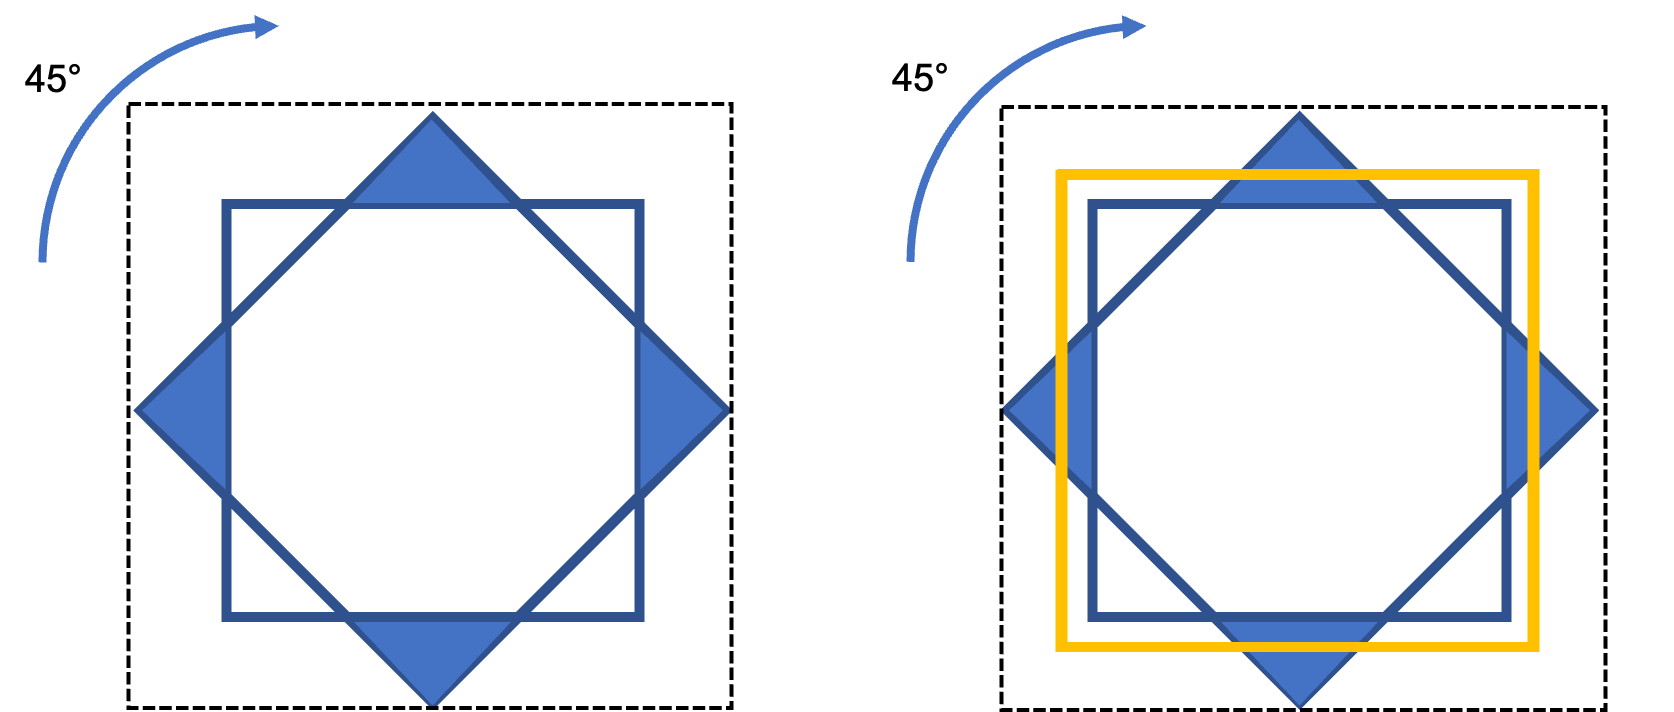
\includegraphics[width=12cm,keepaspectratio]{images/rotation_issue.png}
        \caption{Issue with ear rotation and our solution using zoom on the image with padding.}
    \end{center}
\end{figure}

In order to facilitate a fair comparison, we decided to make all processed images to the same output size,
and for what concerns the corner value of the output image, we opted for pixel interpolation using
neighboring values.
However, even though interpolation seems a reasonable choice, it will introduce noise into the processed image.
We tackle this problem using the aforementioned padding on the input image, but now we also know how much
padding was previously added: we have a way of reducing the noise introduced by interpolation. The idea is
represented in Figure 7. We now apply rotation on a bigger image than the original ROI, then interpolate
values on the corners, and finally "zoom in" in the ear zone (i.e. the area within the orange bounding box)
by applying cropping with a value of zoom that is proportional to the applied padding.

\begin{figure}[h]
    \label{fig:rotation_comparison}
    \begin{center}
        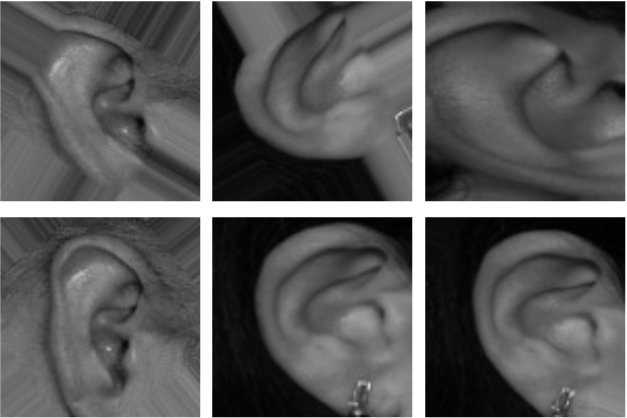
\includegraphics[width=10cm,keepaspectratio]{images/rotation_comparison.png}
        \caption{Interpolation on the corners without (above) and with (below) padding.}
    \end{center}
\end{figure}

\section{Feature extraction phase}

It is a vital phase since we care about representing points of interest in a feature descriptor no matter
where these features are present in our image. In other words, we want to able to extract ear features
even if they appear translated in the original image, then when we perform the matching between descriptors
they should be designed in a way such that they are invariant to such geometric transformations.
For these reasons, we have chosen to rely on the ORB algorithm for the feature extraction task too.
In particular, we found it useful to have a compact feature vector for each detected key point but also
because it allowed us to experiment with a few configurations of the algorithm in order to get the best
results. We experimentally found that using $edgeThreshold=10$ in conjunction with the previous technique
to reduce the points sparsity, allowed us to get a good set of points on the ear shape.
Finally, we performed feature descriptor matching using the $BFMatcher$ that is essentially a brute force
matcher that takes every descriptor in the first and matches it with all the descriptors in the second set.
Once the matching operation is completed, we have a way of measuring distances between the set of descriptors
of the probe image with respect to the current template in the gallery. To reject poor matches and to obtain
a single similarity score, we relied on the ratio test proposed by Lowe et al. \cite{Lowe:2004:DIF:993451.996342}
using a value for $ratio=0.75$, then the similarity between two sets of descriptors is the ratio between good
matches over the total number of matches.

\section{Evaluation phase}

\blindtext

\begin{figure}[H]
    \label{fig:roc}
    \begin{center}
        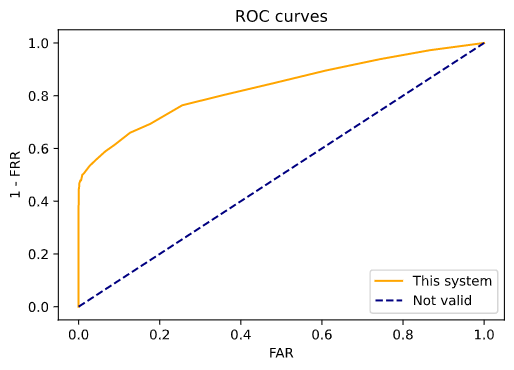
\includegraphics[width=10cm,keepaspectratio]{images/roc.png}
        \caption{Interpolation on the corners without (above) and with (below) padding.}
    \end{center}
\end{figure}

\blindtext

\begin{figure}[H]
    \label{fig:det}
    \begin{center}
        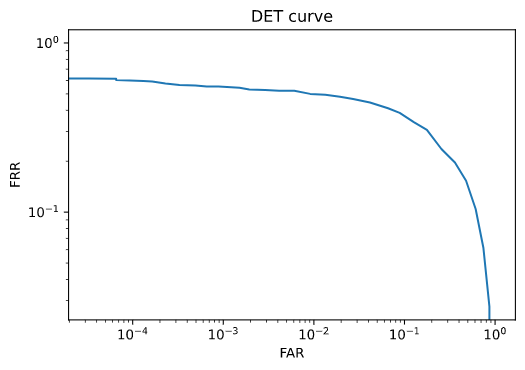
\includegraphics[width=10cm,keepaspectratio]{images/det.png}
        \caption{Interpolation on the corners without (above) and with (below) padding.}
    \end{center}
\end{figure}

\blindtext

\begin{figure}[H]
    \label{fig:eer}
    \begin{center}
        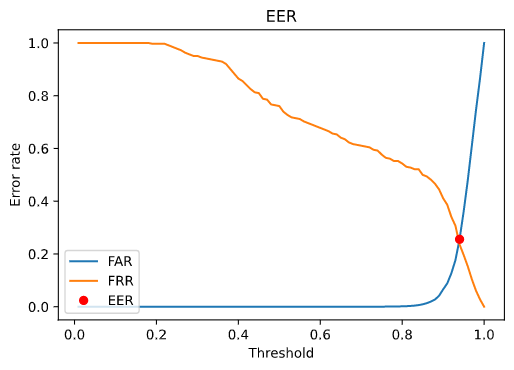
\includegraphics[width=10cm,keepaspectratio]{images/eer.png}
        \caption{Interpolation on the corners without (above) and with (below) padding.}
    \end{center}
\end{figure}

\blindtext

\section{Android porting}

In this work, we implemented the recognition pipeline as a standalone C++ program that was used for
testing the performances of the module on the AMI dataset. We also developed an Android application
to allow the enrollment of new subjects, verification, and identification of already registered ones.
Both the projects heavily rely on the OpenCV library \cite{opencv_library} and have been tested using
version 4.5.1. on both the systems to avoid compatibility issues. The Android project essentially consists
of a porting in the Kotlin language of some of the functionalities available in the desktop application.
The user interface is pretty simple and allows user enrollment via ear image acquisition through the phone
camera. Once acquired, it is passed through our biometric module and processed according to the described pipeline:
the first step is ROI detection using Haar Feature-based Cascade Classifiers, then cropping and resizing with
padding is applied over the obtained area, landmark detection is performed to allow automatic image orientation
along the vertical axis, and finally, the image is rotated according to the computed angle and zoomed in using
the idea which was previously described.
Furthermore, the app allows performing either verification or identification using their dedicated sections.
For the verification task, the user simply declares his claimed identity and selects an image either from the phone
gallery or by taking a photo and submits it to the system. The system will return a decision that is accepted if the
similarity score of the probe image with any of the user templates in the gallery is above the acceptance threshold
or rejected otherwise. On the other hand, the identification tasks will look for matches with any template in the
gallery, check if any template in the gallery generates an alarm for the given input probe, and finally return
the identity associated to the template with the highest similarity score if it is above the considered acceptance
threshold as well as the similarity score.
Moreover, for what concerns the gallery organization we decided to leverage the Android filesystem scheme and
store each template as an individual file named with the id of the corresponding identity. This simple organizational
scheme allows templates to be quickly retrieved whenever necessary and improves project modularity. All the files that
are required for the application to work are shipped with it as bundle files and can be retrieved by using
Android File System API. 

\section{External resources}

In this section we list all the external resources that we used at any step of the pipeline and that are not
built-in in C++/Android or shipped with the base version of the OpenCV library. Their credits are available in
the References section. All of the remaining code or considerations are part of this work and have been
developed during it.

\begin{itemize}
    \item Left and right ear Haar feature-based cascade classifiers from
        the
        \href{https://github.com/DiUS/Physiognomy/tree/master/python/haarcascades}{\emph{official GitHub OpenCV repository}}
        or from
        \href{https://github.com/DiUS/Physiognomy/tree/master/python/haarcascades}{\emph{this repository}}.
    \item First stage landmark detector using a CNN from
        \href{https://github.com/maups/ear-recognition}{\emph{this repository}}.
\end{itemize}

\section{Future work}

This project started with the idea of integrating a distributed database into the Android application to let
enrolled users test verification and identification by submitting their probes with any Android device. Due to
the lack of time, we decided to focus more on the details of the design and implementation of the recognition
process and opted to store locally the gallery in the user's phone. An interesting possibility for this project
would be to integrate such distributed database, for instance using Google Cloud Firestore, to store user templates.
Moreover, we explored multiple approaches for implementing a proper recognition pipeline and a possibility would be
to apply more advanced techniques for landmark detection and feature extraction, for instance training a dedicated
CNN that would probably boost the recognition performances as we saw for the landmark detection phase.

\bibliographystyle{ieeetr}
\bibliography{bibliography}

\end{document}
